% Modelo de relatório no estilo artigo em duas colunas
\documentclass[onecolumn]{article}
\usepackage[utf8]{inputenc}
\usepackage{amsmath}
\usepackage{subcaption}
\usepackage{mathtools}
\usepackage{graphicx}
\usepackage{color}
\usepackage{authblk}
\usepackage{lmodern}
% \usepackage[colorlinks,citecolor=black,urlcolor=black,bookmarks=false,hypertexnames=true]{hyperref}
\usepackage{geometry}
\usepackage{pdfpages}
\usepackage{fancyhdr}
\usepackage[utf8]{inputenc}

\usepackage[sorting=none,style=numeric]{biblatex}
\addbibresource{refs.bib}
\usepackage[justification=centering]{caption}
\usepackage{makecell}
\usepackage{booktabs}
\usepackage{hhline}
\usepackage{amsmath}
\usepackage{amssymb}
\usepackage{soul}
\usepackage{gensymb}
\usepackage{listings}

\setlength\parindent{0pt}


\newcommand{\myname}{Nishant Aswani}
\newcommand{\mynetid}{nsa325}
\newcommand{\myemail}{nsa325@nyu.edu}
\newcommand{\myhwtype}{Mini-Project }
\newcommand{\myhwnum}{1}
\newcommand{\mycoursenumber}{ENGR-UH 4560}
\newcommand{\myclassname}{Selected	Topics	in	Information	
and	Computational Systems: Machine Learning}
\newcommand{\myassignmenttitle}{Climate Change Data Prediction and Modifying Gradient Descent}
\newcommand{\myinstructor}{Hwasoo Yeo}

\newcommand{\cc}[1]{\texttt{#1}}

\lstset{
  basicstyle=\ttfamily,
  escapeinside=||
}

% Tamanho das margens:
\geometry{
 a4paper,
 total={170mm,257mm},
 left=20mm,
 top=20mm,
 }
%%%%%%%%%%%%%%%%%%%%%%%%%%%%%%%%%%%%%%%%%
% Bibliografia estilo ABNT. Se não tiver instalado, comente a linha abaixo.
% \usepackage[alf, abnt-etal-list=0, abnt-emphasize=bf,abnt-last-names=bibtex, abnt-etal-text=it, abnt-etal-cite=2]{abntex2cite}
%%%%%%%%%%%%%%%%%%%%%%%%%%%%%%%%%%%%%%%%%

% Dados de identificação
\title{\myassignmenttitle}
\author{\myname, \myemail}
\affil{ \myclassname  (\mycoursenumber), Professor \myinstructor}
\date{}

\begin{document}
%%%%%%%%%%%%%%%%%%%%%%%%%%%%%%%%%%%%%%%%%%%%%%%% COVER PAGE %%%%%%%%%%%%%%%%%%%%%%%%%%%%%%%%%%%%%%%%%%%%%%%%%%%%
\onecolumn
\pagestyle{fancy}
\fancyhf{}
\renewcommand{\headrulewidth}{0pt}
\onecolumn

\rhead{\textbf{Division of Engineering}}
\lhead{\textbf{NYU Abu Dhabi}}

\begin{center}
  
\includegraphics[scale=0.20]{etc/NYUAD-alt-logo.jpg}
\end{center}

{\vspace{2.5em}}

\begin{center}
    \Huge{\textbf{\mycoursenumber}}\\
    {\vspace{0.5em}}
    \Huge{\textbf{\myclassname}}
\end{center}

{\vspace{5em}}

\begin{center}
  \begin{tabular}{|rp{5.0cm}lll|}
    \hline
    &  &  &  & \\
    &  &  &  & \\
    \Large{\textbf{Name:}} & \Large{\myname}
    
    \  &  &  & \\
    \Large{\textbf{Net ID:}} & \Large{\mynetid}
    
    \  &  &  & \\
    \Large{\textbf{Assignment Title:}} & \Large{\myhwtype \myhwnum}
    
    \
    
    \  &  &  & \\
    \hline
  \end{tabular}
\end{center}

\
{\newpage}
%%%%%%%%%%%%%%%%%%%%%%%%%%%%%%%%%%%%%%%%%%%%%%%% COVER PAGE %%%%%%%%%%%%%%%%%%%%%%%%%%%%%%%%%%%%%%%%%%%%%%%%%%%%
\onecolumn
\maketitle        

% Resumo de no máximo 200 palavras
% \begin{abstract}
% Este documento orienta a descrição das atividades práticas desenvolvidas em laboratório. São usados como exemplo conceitos da Aula 01 de Acionamentos Elétricos sobre partida direta de motor de indução trifásico. Nesta atividade, um motor é acionado com conexões estrela e triângulo a vazio. As correntes nominais e de partida são medidas com amperímetro analógico e comparadas entre si. Nota-se que, mesmo sem carga, as corrente em estrela são maiores. 
% \end{abstract}
\vspace{-5mm}
\section{Introduction}

The Gradient Descent Method is an iterative method used to find the minimum of a given function. In this mini project, modifications are made to the standard stochastic gradient descent method to minimize the cost function and obtain a linear model for socioeconomic factors affecting city emissions. The report also discusses the reasons for these modifications and its practical use.\\ 

The dataset was obtained from a Nature article titled "A global dataset of CO2 emissions and ancillary data related to emissions for 343 cities" authored by Nangini et. al \cite{nangini2019global}. The authors gathered emissions and ancillary data for 343 cities from a variety of sources, carried out data quality control, and combined it to form a dataset. The data covers "data from CDP (187 cities, few in developing countries), the Bonn Center for Local Climate Action and Reporting (73 cities, mainly in developing countries), and data collected by Peking University (83 cities in China)" \cite{nangini2019global}.

\section{Methodology}

\subsection{Data Selection}

As there was Scope 1 Green House Gas (GHG) Emissions data available for all 343 cities, it was selected to be the target variable. Scope 1 GHGs refer to "transport, industrial, waste and local power plants emissions" \cite{nangini2019global}. \\

From the larger dataset, a small range of potentially interesting features were initially selected. Using a heatmap, the two most interesting features were selected: Population and Built-up Area. \\

Data verification for the target variable showed that there was an extreme outlier; for simplicity, this row was dropped out of the dataframe. Moreover, all rows with unavailable, or \cc{NaN} values, were dropped.  

\subsection{Data Preprocessing}

Since ""[learning estimators] might behave badly if the individual features do not more or less look like standard normally distributed data," \cite{sklearnpreprocessing} the data was preprocessed using sklearn's RobustScaler method. The result of standardization can be seen below in kernel density estimation (KDE) plot. Furthermore, the dataset was split into training (80\%) and testing (20\%).

\begingroup
    \centering
    \medskip
    %width=\columnwidth
    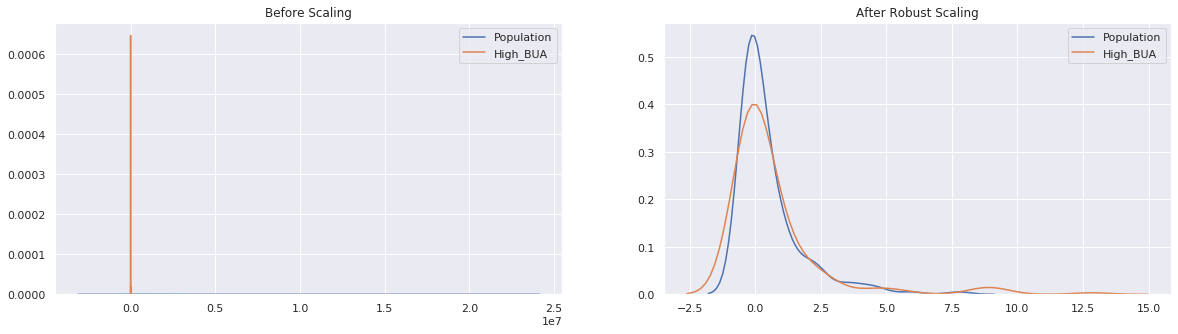
\includegraphics[width=\columnwidth]{Tex/mp1_images/scaling.png}
    \captionof{figure}{Before and after standardization of the features}
    \medskip
\endgroup
\medskip


\subsection{Gradient Descent}

As a benchmark to compare gradient descent methods, the built-in sklearn linear regression model was used to train standardized training data set.Next, a model was trained using a standard stochastic gradient descent, with a rational function as the learning schedule. \\

The modified gradient descent sought to tweak two of the core functionalities: the learning schedule and determination of the gradient.

\subsubsection{Learning Schedule}

The original learning schedule is a rational function $\frac{t_{0}}{t+t_{1}}$, where t is updated at each iteration. The hyperparameters $t_0$ and $t_1$ are selected so that at $t = 0$, the learning rate is 0.1. The learning rate then rapidly decreases until it plateaus towards the end. \\

Initially, it was thought to update the learning schedule's hyperparameters so that learning reflected the depth or shallowness of the cost function parabaloid. However, it was realized that $\theta$ does account for the gradient at each iteration. Hence, factoring the gradient into the learning schedule might over or underplay its effect in calculating the next $\theta$ value. \\

Often, gradient descent methods face the challenge of finding themselves stuck at local minima instead of converging at the global minima. Hence, the modified gradient descent attempted to use a linearly descending, dampened sine wave to "shock" the model out of local minima situations. A dampened-sin wave function was derived for a given epochs of 50. \\

It is clear that the goal of the original learning schedule is to aid in converging as rapidly as possible and then tweak the model slowly. On the other hand, the dampened sin wave initially provides larger shocks to the system and then gradually converts into a negative linear slope.\\

\begingroup
    \centering
    \medskip
    %width=\columnwidth
    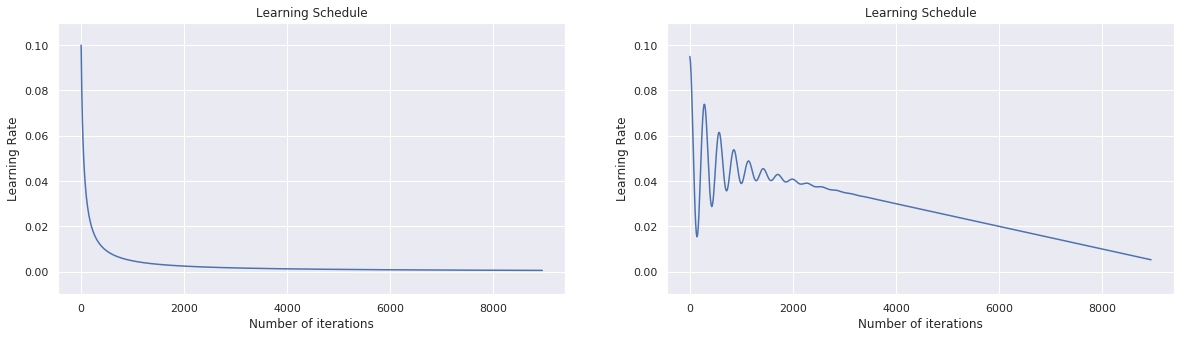
\includegraphics[width=\columnwidth]{Tex/mp1_images/schedule.png}
    \captionof{figure}{The original learning schedule compared with the modified learning schedule}
    \medskip
\endgroup
\medskip

A variation of the dampened sin wave was initially considered, pictured at the bottom-right. However, the model was discarded as it provided too large of a variation even towards the end of the iterations.\\

\begingroup
    \centering
    \medskip
    %width=\columnwidth
    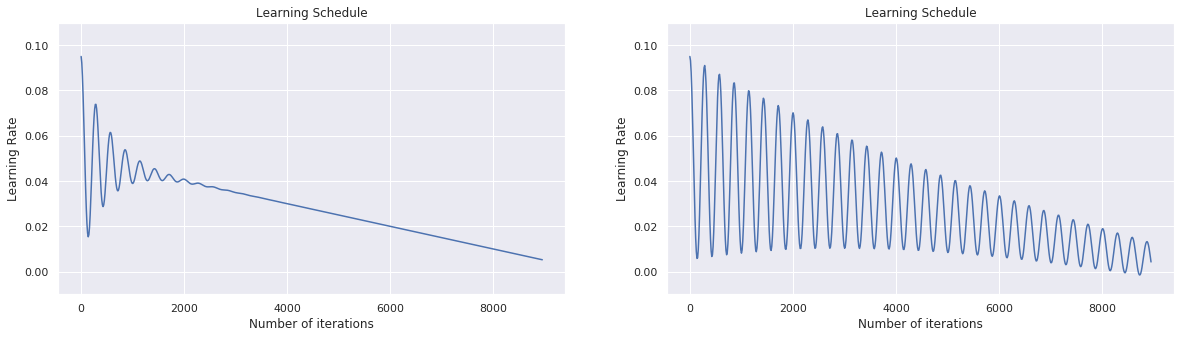
\includegraphics[width=\columnwidth]{Tex/mp1_images/schedule2.png}
    \captionof{figure}{The original learning schedule compared with the modified learning schedule}
    \medskip
\endgroup
\medskip

However, in the case of linear regression there is no concern for being stuck at local minima, as there is only one minimum to which the model must converge to.

\subsubsection{Gradient Averaging}

Another modification made was the method of determining the gradient. It was realized that gradient calculation was reliant upon the random selection of a data point from the training data. To modify gradient calculation, the training space was divided into three sections. In each iteration, three random data points were selected, one from each of the split sections. \\

\begingroup
    \centering
    \medskip
    %width=\columnwidth
    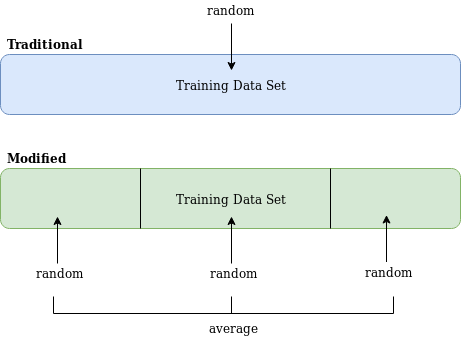
\includegraphics[width=0.4\columnwidth]{Tex/mp1_images/avg.png}
    \captionof{figure}{Gradient averaging, where the pipe represents finding the gradient of the random datapoint}
    \medskip
\endgroup
\medskip

Since sklearn's train test splitting method randomizes the data after splitting, there was no fear of data bias. The gradient of each of the three data points was calculated and averaged to obtain a single gradient value for each feature. As before, this was used to update the theta. In reality, splitting the data into three section has little effect, aside from increasing the probability of each data point being selected. However, selecting an average gradient of several random points, instead of just one, prevents an unreasonably large gradient from affecting the step size. \\

The reason for why averaging the gradient works lies in understanding that the derivative of a sum of functions is equal to the sum of a derivative functions.

\section{Results}

For this project, the built-in \cc{LinearRegression} method was used as a benchmark to compare the unmodified and modified gradient descent (GD) approaches. The table below shows the results of 100 runs of each method.\\

\begingroup
    \medskip
    \centering
    \def\arraystretch{1.5}
        \begin{tabular}{lccccc}
            \toprule
            Method & Pop. Coeff. & Pop. Coeff. Variance & BUA Coeff. & BUA. Coeff. Variance & Time(s)\\
            \midrule
            sklearn LinReg & 0.776708 & N/A & 0.294042 & N/A & N/A\\
            Traditional SGD          & 0.779071 & 0.00314603 & 0.29797795 & 0.00159789 & 8.15\\
            Modified SGD             & 0.77412671 & 0.00112532 & 0.2980754 & 0.00071944 & 39.2\\
            \bottomrule
        \end{tabular}
    \captionof{table}{Execution statistics comparing the two GD methods}
    \label{fig:c2table1}
    \medskip
\endgroup

From the modified method, we are given the model, where we can use the intercept determined by sklearn to replace the bias term:\\

\begin{equation}
    \begin{split}
        y & = 0.015627 + 0.77412671x_{1} + 0.2980754x_{2}\\
    \end{split}
    \label{eq:turns}
\end{equation}

\newpage

\section{Discussions and Conclusion}

As shown by the results, the traditional method has a higher variance compared to the modified method. We can thus infer that the modified method is more likely to converge at the minimum. However, at 100 iterations, the modified method is approximately five times slower. This is because the modified method runs an extra for-loop, decreasing convergence time.\\ 

Moreover, the learning rate used in the modified method would be more applicable for problems beyond linear regression, where being trapped within a local minima would pose as a real risk. Another drawback of the learning rate is that it would have to be re-crafted if the number of epochs were to change because the dampened sin wave is a sensitive function.\\

Overall, the modified method trades-off convergence time for likelihood of convergence, which could be useful depending on the resources at hand and endgoal. 


%%%%%%%%%%%%%%%%%%%%%%%%%%5
% BIBLIOGRAFIA 
% Estilo de bibliografia ABNT. Se não tiver instalado, mude para plain ou ieeetr

%\bibliographystyle{plain} % Inclua isso se não tiver ABNTEX instalado
% \begin{thebibliography}{refs}
% \bibitem{}
\printbibliography
% \end{thebibliography}
\end{document}